\clearpage % clear the prior chapter's page

\chapter{Supplement to "Rapid simulation of unprocessed DEER decay data for protein fold prediction"} \label{app:rosettadeer_supp}
%\vspace{-7mm}
%\bigskip

This Appendix contains supplementary information for Chapter \ref{ch:rosettadeer}.

\begin{table}[h!]
\scriptsize
\renewcommand{\tabcolsep}{0.09cm}
\centering
\caption[List of spin-labeled proteins in the Protein Databank.]{List of spin-labeled proteins in the Protein Databank.}

\newcolumntype{Y}{>{\raggedright\arraybackslash}X}

\begin{center}
\begin{tabular}{l l l l r}
\toprule \\
\textbf{Protein} & \textbf{PDB} & \textbf{Angle} & \textbf{Distance} & \textbf{Ref.} \\
T4 Lysozyme & 1ZYTa & 5.23  & 0.83 & \citep*{Fleissner2009} \\
T4 Lysozyme & 2CUUa & 7.24  & 0.84 & \citep*{Fleissner2009} \\
T4 Lysozyme & 2CUUa & 3.39  & 0.78 & \citep*{Fleissner2009} \\
T4 Lysozyme & 2IGCa & 11.49 & 0.81 & \citep*{Guo2008} \\      
T4 Lysozyme & 2NTHa & 3.06  & 0.8  & \citep*{Guo2008} \\      
T4 Lysozyme & 2OU8a & 7.13  & 0.82 & \citep*{Guo2008} \\      
T4 Lysozyme & 2OU8a & 9.08 & 0.86 & \citep*{Guo2008} \\      
T4 Lysozyme & 2OU9a & 15.13 & 0.84 & \citep*{Guo2008} \\      
T4 Lysozyme & 2Q9Da & 10.99 & 0.8  & \citep*{Guo2008} \\      
T4 Lysozyme & 2Q9Ea & 14.55 & 0.86 & \citep*{Guo2008} \\      
T4 Lysozyme & 2Q9Eb & 14.55 & 0.86 & \citep*{Guo2008} \\      
T4 Lysozyme & 2Q9Ec & 8.08  & 0.84 & \citep*{Guo2008} \\      
GB1         & 3V3Xb & 4.78  & 0.83 & \citep*{Cunningham2012} \\ 
GB1         & 3V3Xb & 8.53  & 0.82 & \citep*{Cunningham2012} \\ 
GB1         & 3V3Xb & 1.13  & 1.02 & \citep*{Cunningham2012} \\ 
GB1         & 3V3Xc & 2     & 0.8  & \citep*{Cunningham2012} \\ 
GB1         & 3V3Xd & 5.65  & 0.78 & \citep*{Cunningham2012} \\ 
GB1         & 3V3Xd & 1.39  & 0.8  & \citep*{Cunningham2012} \\ 
GB1         & 3V3Xd & 2.71  & 0.81 & \citep*{Cunningham2012} \\ 
%P450cam     & 4EK1a & 5.64  & 0.78 & \citep*{Still2012}      \\ 
%P450cam     & 4EK1b & 8.46  & 0.8  & \citep*{Still2012}      \\ 
GB1         & 5BMGa & 10.97 & 1.08 & \citep*{Cunningham2016} \\ 
GB1         & 5BMGb & 4.57  & 0.79 & \citep*{Cunningham2016} \\ 
GB1         & 5BMGc & 13.52 & 1.13 & \citep*{Cunningham2016} \\ 
GB1         & 5BMGd & 5.89  & 0.8  & \citep*{Cunningham2016} \\ 
GB1         & 5BMGe & 1.45  & 0.99 & \citep*{Cunningham2016} \\ 
GB1         & 5BMGf & 7.7   & 0.84 & \citep*{Cunningham2016} \\ 
GB1         & 5BMGg & 8.47  & 0.87 & \citep*{Cunningham2016} \\ 
GB1         & 5BMHa & 8.29  & 0.77 & \citep*{Cunningham2016} \\ 
GB1         & 5BMHa & 9.38  & 0.77 & \citep*{Cunningham2016} \\ 
GB1         & 5BMIa & 7.42  & 0.83 & \citep*{Cunningham2016} \\ 
Azurin      & 5I26a & 4.8   & 0.81 & \citep*{Consentius2016} \\ 
Azurin      & 5I26b & 0.55  & 0.99 & \citep*{Consentius2016} \\ 
Azurin      & 5I26c & 0.92  & 1.01 & \citep*{Consentius2016} \\ 
Azurin      & 5I26d & 0.89  & 1    & \citep*{Consentius2016} \\ 
Azurin      & 5I28a & 0.5   & 1    & \citep*{Consentius2016} \\ 
Azurin      & 5I28b & 0.71  & 1    & \citep*{Consentius2016} \\ 
Azurin      & 5I28c & 0.32  & 1.01 & \citep*{Consentius2016} \\ 
Azurin      & 5I28d & 0.25  & 1.01 & \citep*{Consentius2016} \\ 
Azurin      & 5I28e & 4.49  & 0.96 & \citep*{Consentius2016} \\ 
Azurin      & 5I28f & 1.81  & 1.01 & \citep*{Consentius2016} \\ 
Azurin      & 5I28f & 2.15  & 0.98 & \citep*{Consentius2016} \\ 
Azurin      & 5I28h & 2.1   & 0.89 & \citep*{Consentius2016} \\ 
Azurin      & 5I28i & 5.44  & 0.8  & \citep*{Consentius2016} \\ 
Azurin      & 5I28j & 6.8   & 0.85 & \citep*{Consentius2016} \\ 
T4 Lysozyme & 5JDTa & 2.52  & 0.78 & \citep*{Consentius2016} \\ 
T4 Lysozyme & 5JDTa & 0.85  & 0.76 & \citep*{Consentius2016} \\ 
\bottomrule \\
\end{tabular} 
\end{center}
\label{tab:rosettadeer_main_slproteins}
\end{table}

\begin{figure}[h]
\centering
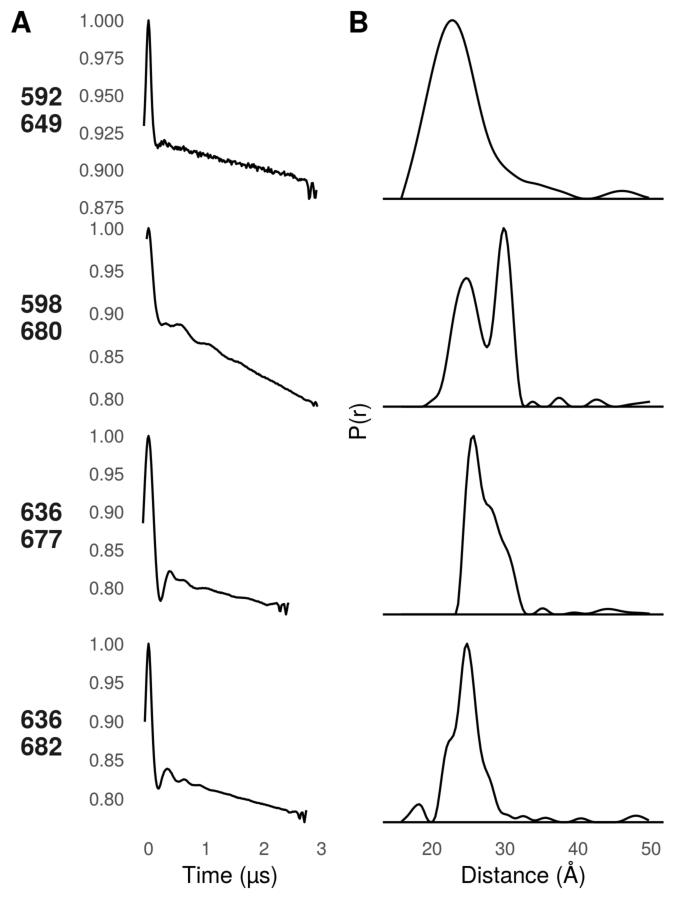
\includegraphics[width=4in]{Figures/rosettadeer_supp_exou.pdf}
 \caption[Data gathered in the ExoU C-terminus for this study.]{Data gathered in the ExoU C-terminus for this study.}
\label{fig:rosettadeer_supp_exou}
\end{figure}

\begin{figure}[h]
\centering
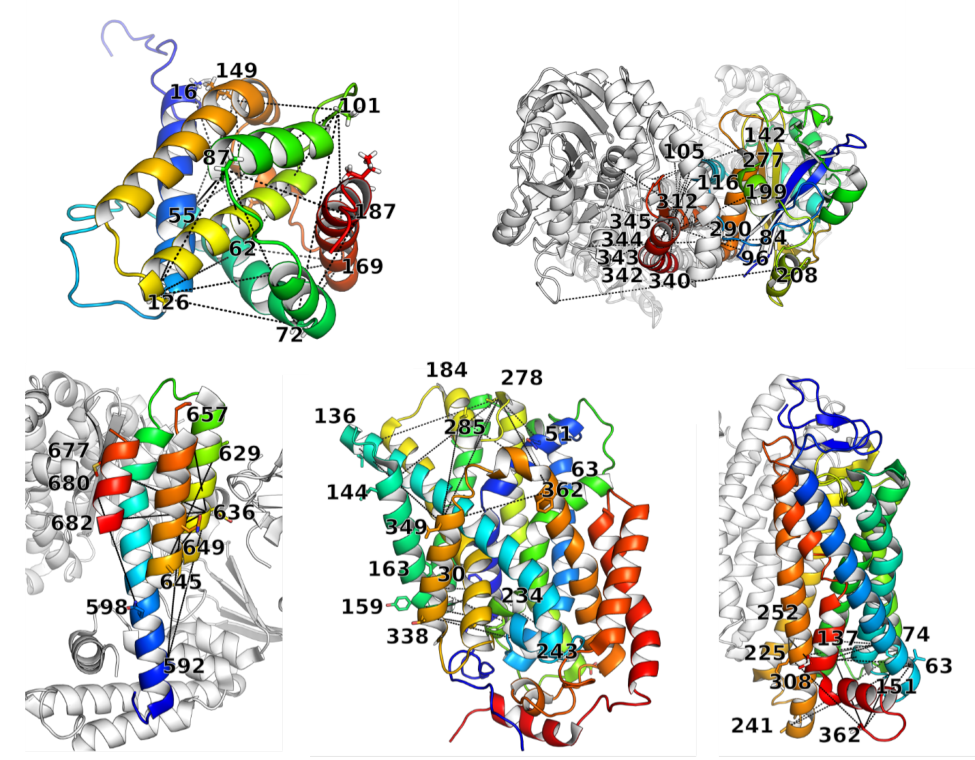
\includegraphics[width=5.5in]{Figures/rosettadeer_supp_restraints.pdf}
 \caption[Placement of experimental DEER restraints on protein structures used in this study.]{Placement of experimental DEER restraints on protein structures used in this study. Clockwise from top left: Bax (PDB: 1F16 model 8), CDB3 (PDB: 1HYN chains R/S), Rhodopsin (1GZM chain A), Mhp1 (PDB: 2JLN), and ExoU (PDB: 3TU3, C-terminus only).}
\label{fig:rosettadeer_supp_restraints}
\end{figure}

\begin{figure}[h]
\centering
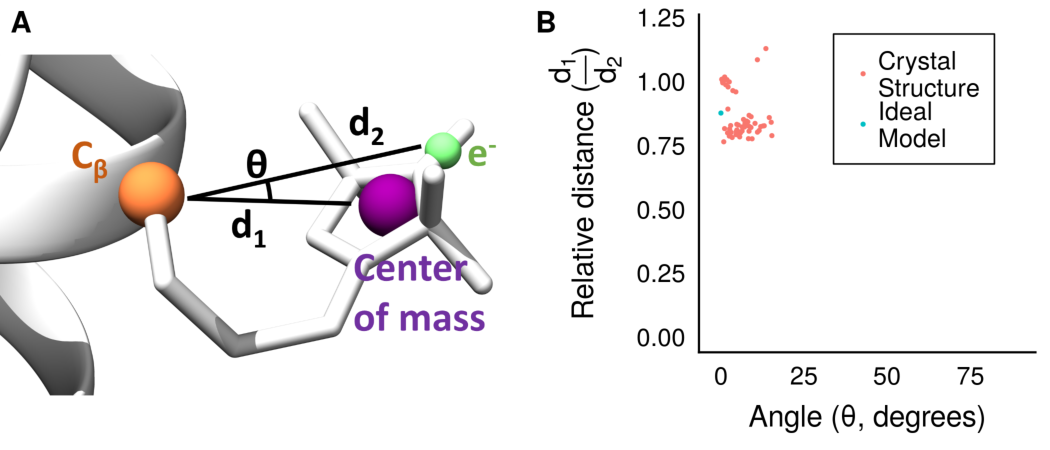
\includegraphics[width=6in]{Figures/rosettadeer_supp_sl.pdf}
 \caption[Nitroxide centers of mass fall along the $\mathrm{C_{\upbeta}}$-electron vector.]{Nitroxide centers of mass fall along the $\mathrm{C_{\upbeta}}$-electron vector. A) Depiction of spin label from PDB: 2Q9D showing the nitroxide center of mass (purple) and the nitroxide bond midpoint (green). B). Angle and relative distance of nitroxide center of mass along the $\mathrm{C_{\upbeta}}$-electron vector.}
\label{fig:rosettadeer_supp_sl}
\end{figure}

\begin{figure}[h]
\centering
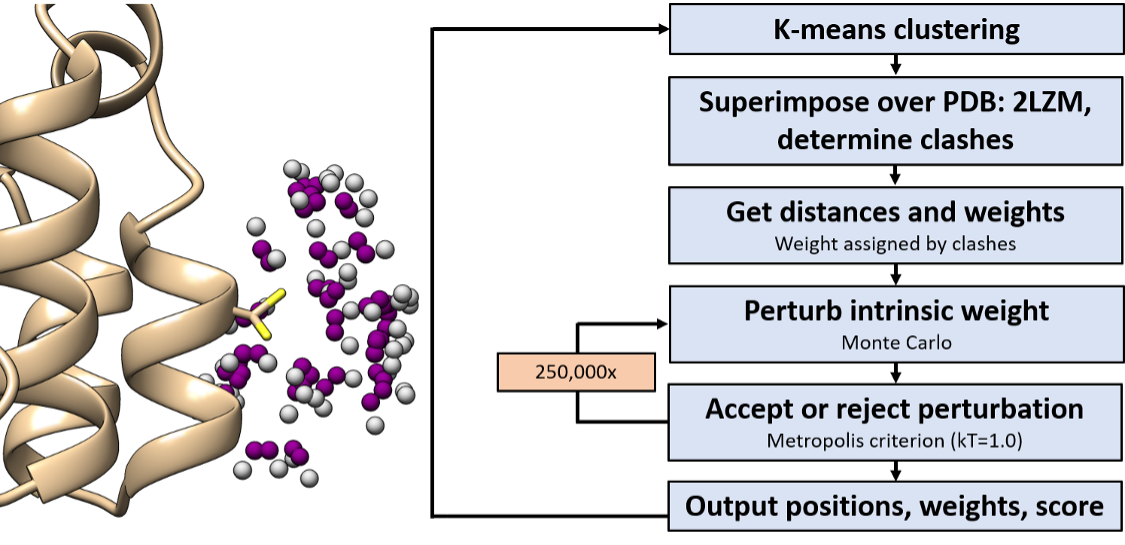
\includegraphics[width=6in]{Figures/rosettadeer_supp_scheme.pdf}
 \caption[Optimization of RosettaDEER measurement coordinates.]{Optimization of RosettaDEER measurement coordinates. Left: Each of the rotamers in Rosetta’s \gls{mtssl} rotamer library was converted into two coordinates: one representing the nitroxide ring center of mass (purple), which was used to evaluate clashes; and one representing the nitroxide bond midpoint (silver), from which distances were measured. Shown over PDB 2CUU residue 131. Right: Optimization scheme for reducing the number of measurement coordinates using experimental T4 Lysozyme distance data. One thousand replicates were performed for each of N clusters, with N ranging from 3 to 53 coordinates.}
\label{fig:rosettadeer_supp_scheme}
\end{figure}

\begin{figure}[h]
\centering
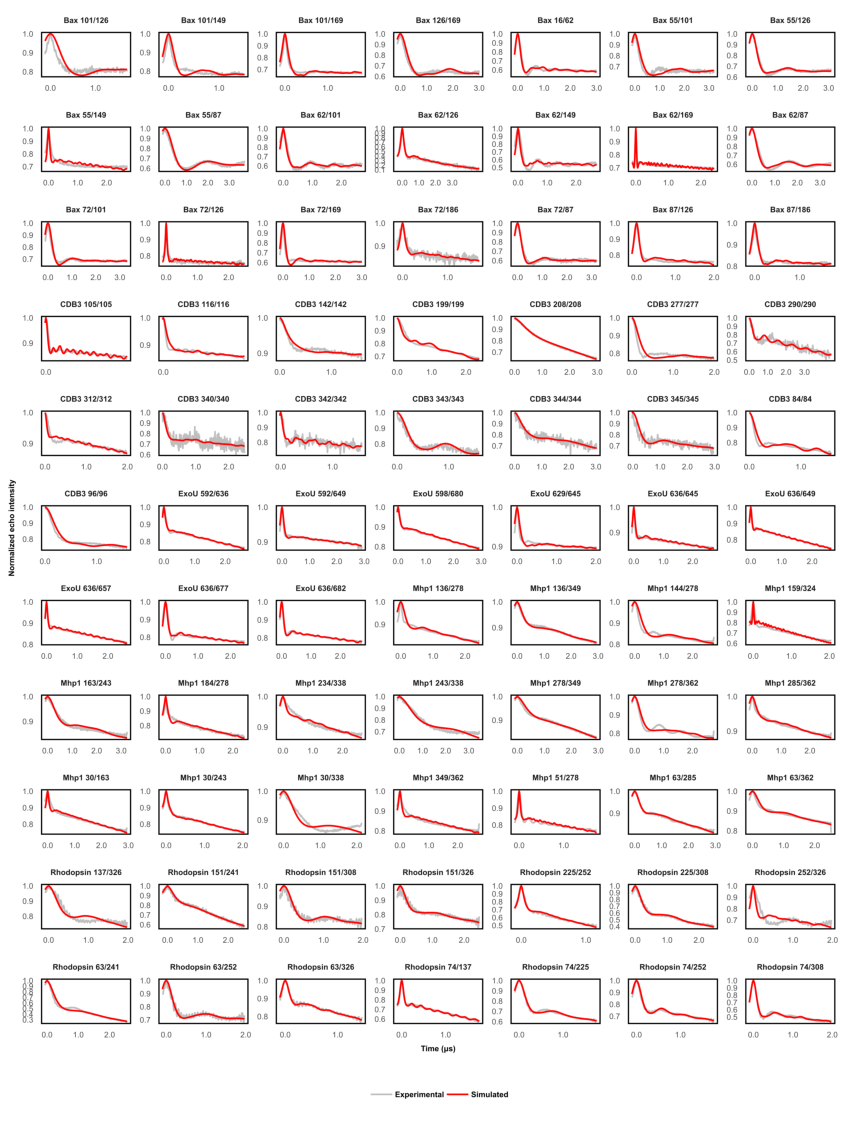
\includegraphics[width=5.5in]{Figures/rosettadeer_supp_alltraces.pdf}
 \caption[All simulated and experimental DEER decay data used in this study between experimentally resolved residues.]{All simulated and experimental DEER decay data used in this study between experimentally resolved residues. RosettaDEER could generally, but not always, simulate DEER traces from native-like models that are comparable to the experimental data.}
\label{fig:rosettadeer_supp_alltraces}
\end{figure}

\begin{figure}[h]
\centering
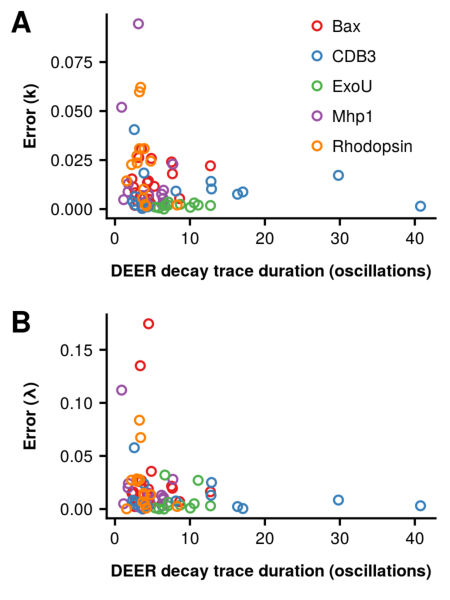
\includegraphics[width=3in]{Figures/rosettadeer_supp_oscillations.pdf}
 \caption[Deviation between experimental and simulated background decay ($k$) and modulation depths ($\lambda$).]{Deviation between experimental and simulated background decay ($k$) and modulation depths ($\lambda$).}
\label{fig:rosettadeer_supp_oscillations}
\end{figure}

\begin{figure}[h]
\centering
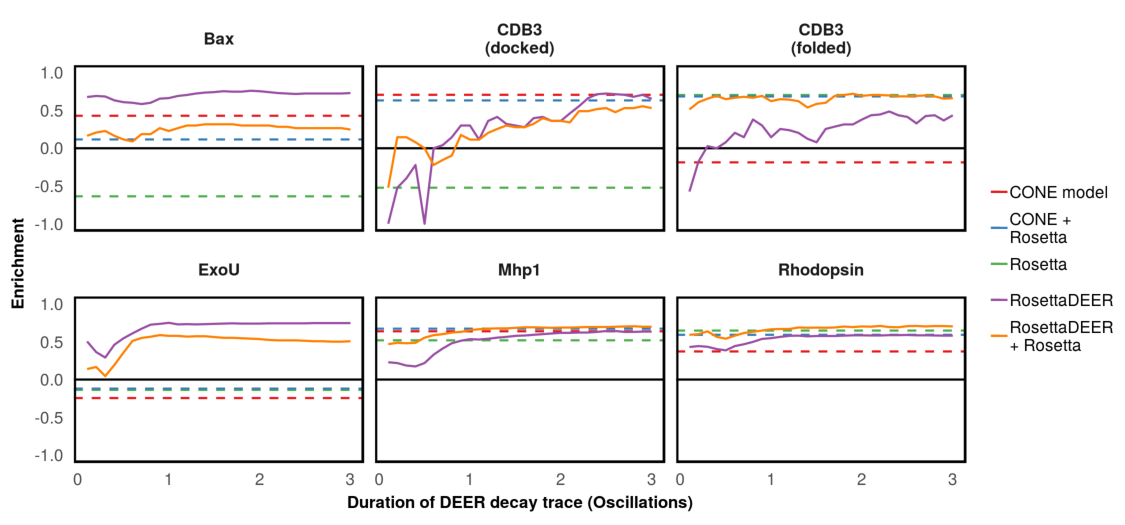
\includegraphics[width=5.5in]{Figures/rosettadeer_supp_oscillation_decoys.pdf}
 \caption[Enrichment of misfolded and misdocked decoys as a function of DEER decay trace duration.]{Enrichment of misfolded and misdocked decoys as a function of DEER decay trace duration. Enrichment was quantified as the logarithm of the percentage of native-like models (top 10\% by $\mathrm{RMSD_{100SSE}}$) that were also in the top 10\% by score. An enrichment of 1 indicates that the set of models constituting the top 10\% by RosettaDEER score was identical to the set of models constituting the top 10\% by Rosetta score.}
\label{fig:rosettadeer_supp_oscillation_decoys}
\end{figure}

\begin{figure}[h]
\centering
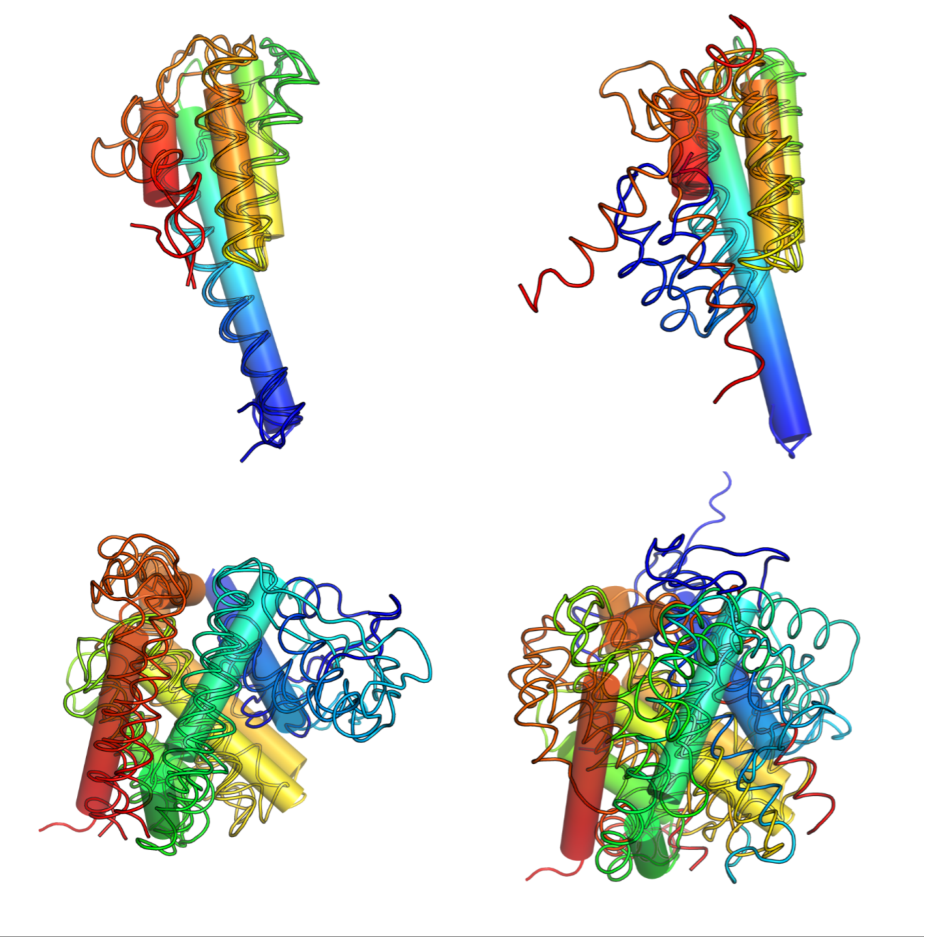
\includegraphics[width=5.5in]{Figures/rosettadeer_supp_top3.pdf}
 \caption[Effect of DEER restraints on structure prediction of Bax and ExoU. ]{Effect of DEER restraints on structure prediction of Bax and ExoU. Top 3 best-scoring models of ExoU (top) and Bax (bottom) folded either with (left) or without (right) experimental \gls{deer} restraints. The native models are shown as cylinders for comparison.}
\label{fig:rosettadeer_supp_top3}
\end{figure}

%\vspace{-7mm}
\bigskip
